\section{NAPLab}

\todo[inline]{denne delen er en draft}

This thesis was done in collaboration with \acrfull{naplab}, a research group at NTNU with the objective of continuously developing and researching state-of-the-art models for autonomous vehicles that are robust to a Nordic environment \cite{naplab}. 

\subsection{NAPLab car}
 NAPLab owns a 2019(?) Kia e-Niro modified to be used for autonomous driving research. The car is equipped with three LIDARs (roof, front and rear right), eight cameras (three in front, two on each side mirror and one in the back), two Radars (front and rear), two GNSS antennas on the roof and four 4G/5G antennas (two in the front window, two on each rear side window). \cref{fig:kia-sensors} show the placements of the camera and LIDAR sensors. The relevant sensors for this thesis are the top LIDAR and the front and side cameras.

 \begin{figure}[htbp]
    \centering
    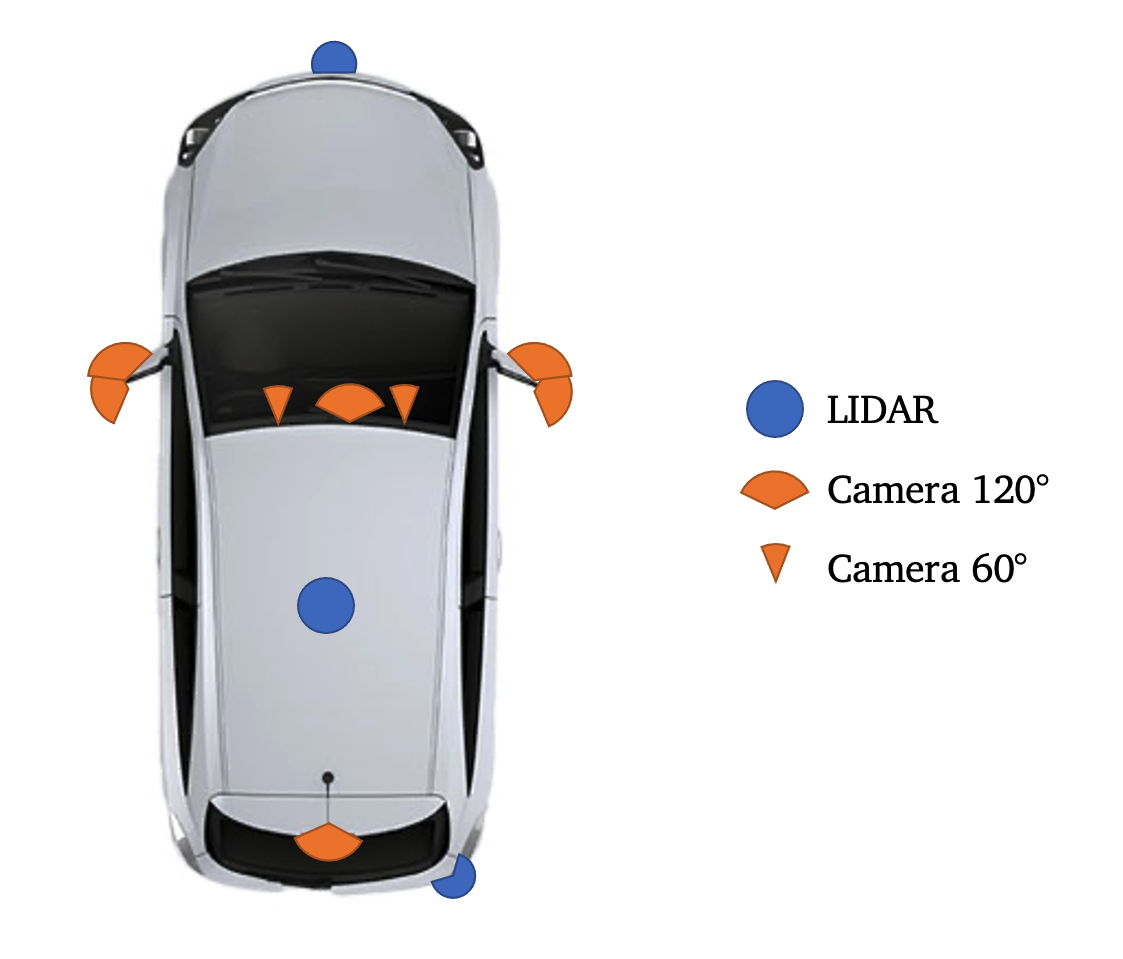
\includegraphics[width=.8\textwidth]{chapters/2-background/figures/kia-sensors.png}
    \caption{Placements of the LIDAR and camera sensors on NAPLab's Kia e-Niro.}
    \label{fig:kia-sensors}
\end{figure}
